\documentclass[conference,a4paper]{IEEEtran}
\IEEEoverridecommandlockouts
% The preceding line is only needed to identify funding in the first footnote. If that is unneeded, please comment it out.
%Template version as of 6/27/2024

\usepackage{cite}
\usepackage{amsmath,amssymb,amsfonts}
\usepackage{algorithmic}
\usepackage{graphicx}

\usepackage{textcomp}
\usepackage{tikz}
\usepackage{booktabs}
\usepackage{xcolor}
\usepackage{hyperref}
\usepackage{array}
\usepackage{tabularx}
\usepackage{amssymb} 


\def\BibTeX{{\rm B\kern-.05em{\sc i\kern-.025em b}\kern-.08em
    T\kern-.1667em\lower.7ex\hbox{E}\kern-.125emX}}
\begin{document}

% Custom figure command: pass filename and caption
\newcommand{\cfigure}[2]{%
  \begin{figure}[h]
    \centering
    \includegraphics[width=\linewidth]{figures/#1.png}%
    \caption{#2}%
    \label{fig:#1}%
  \end{figure}%

}
\title{Summary of Potential of artificial intelligence in reducing energy and carbon emissions of commercial buildings at scale}

\author{Dwayne Mark (Dwayne) Acosta \\ Mohamed Amine (Mohamed) Benaziza \\ David Franz \\ Ray Marange \\ James Thompson\\
\textit{Victoria University of Wellington}\\}
\date{\today}

\maketitle

\section*{Introduction}
\textit{Summary by Ray Marange}
Ding et Al\footcite{dingPotentialArtificialIntelligence2024} explores the potential for AI \dots.

Climate change is accelerating, and buildings are a major contributor, responsible for 39\% of U.S. primary energy use. With urbanization surging and building stock/demand expected to double by 2060, improving building efficiency is no longer optional but urgent.
While AI has transformed industries such as healthcare and finance, its potential in building energy efficiency remains underexplored. AI demonstrates significant potential to reduce costs, enhance benefits, and improve safety across the building lifecycle. This study investigates how AI can reduce energy consumption and carbon emissions in medium-sized office buildings, offering a scalable framework that could be applied globally.
We will explore four key areas: \textbf{Results}, \textbf{Discussion}, \textbf{Methods}, and \textbf{Takeaways \& Reflections}. The study focuses on medium-sized offices, and the results can be extrapolated to offices of any size.
\end{frame}

\section*{AI's impact on energy and emission reductions}
\textit{Summary by Dwayne Mark Acosta}

According to the 2012 U.S. Energy Information Association (EIA) survey, office buildings have the highest energy consumption among commercial types (20\%), with a median energy use intensity (EUI) of 167~kWh/m\textsuperscript{2} (EUI\textsubscript{base}). In contrast, 67 verified low-energy office buildings reported a median EUI of 57~kWh/m\textsuperscript{2} (EUI\textsubscript{HEEB}). The difference between the baseline and best practice energy performance yields a technical energy efficiency saving (TEES) of 110~kWh/m\textsuperscript{2}. TEES can be improved in four categories: equipment, occupancy influence, control and operation, and design and construction.

This study focuses on medium office buildings, which comprise 70\% of total office energy use. The Department of Energy's (DOE) EnergyPlus tool, defined by ASHRAE Standard 90.1, was used to simulate the annual building energy consumption of medium office buildings across four climate zones using representative U.S. cities. Both electricity and natural gas use were considered, with gas assumed to supply hot water and heating. 

To estimate the TEES, a set of 23 improvement cases was developed by varying key design parameters. These include 8 cases for equipment efficiency, 9 for design and construction, and 6 for occupancy-related behavior and control. The cases, based on conservative assumptions, are summarized in Table~\ref{tab:all-cases}, and their contributions to total annual energy savings across different climate zones are illustrated in Figure~\ref{fig:category-breakdown}. The results represent the maximum technical potential achievable through simulation, achieving these savings in practice may require substantial effort throughout the building lifecycle. AI technologies such as fault detection, smart sensors, robotic construction and others can help automate and streamline this process at lower cost and reduced labor.

\textit{Key Takeaway/Thoughts:} Although simulation results suggest that TEES across the four categories can range from 6\% to 27\%, the paper assumes highly optimized performance which requires significant time, resources, and coordination across the building lifecycle. This idealized level of optimization is often difficult to achieve in practice due to real-world constraints. While AI tools may support these optimizations, their practical effectiveness is not guaranteed and remains highly dependent on a wide range of factors including data quality, user adoption, and integration with current systems.



\section*{AI's impact on energy and emission reductions}
\textit{Summary by Dwayne Mark Acosta}

\section*{AI's reduces emissions of buildings}
\textit{Summary by David Franz}

\subsection*{Primary focus of modeling}

The paper focuses on two ways that AI can reduce the emissions of buildings.

\begin{enumerate}
    \item By helping scale up the technologies and speed adoption by reducing the construction and labor costs;
    \item By helping reduce emissions in ongoing maintenance and any new construction over the entire building's lifetime.
\end{enumerate}

\\

\subsection*{Scenarios simulated}
The paper uses the results gained from the previous section to \textbf{simulate six scenarios}. The data is used to estimate parameters for use with complex simulation software to attempt to model the potential lifetime impact on emissions.
\begin{enumerate}
    \item Frozen with current building efficiency;
    \item BAU without AI;
    \item BAU with AI;
    \item Three policy-driven scenarios promoting high-efficiency energy buildings and net-zero energy buildings, and other policy implementation to achieve zero emissions by 2050.
\end{enumerate}

\\

\subsection*{Simulation results}
The results of the simulation are shown below.

Table \ref{tab:energy-emissions} shows the energy use and CO$_2$ emissions for different scenarios.

\begin{table}
\centering
\begin{tabular}{|c|c|c|}
\hline
\textbf{Scenario} & \textbf{Energy Use (kWh/m$^2$)} & \textbf{CO$_2$ Emissions (kg/m$^2$)} \\
\hline 
Baseline & 200 & 50 \\
\hline
AI Optimized & 150 & 30 \\
\hline
\end{tabular}
\label{tab:energy-emissions}
\end{table}

\cfigure{cool-figure}{Different energy use scenarios.}

\\

\subsection*{Key insight}

\textit{“The scenario with AI leads to a higher market share of HEEBs and NZEBs over time compared with the scenario without AI. This trend continues until the market share of net NZEBs reaches its maximum share.”}

The paper asserts that using AI in the ways that they propose always leads to a higher market share of efficient buildings. 

\\

\subsection*{Thoughts on result}
The paper examines various scenarios with some amount of estimation for unknowns, so each individual simulation is unlikely to be exactly right. However, the fact that all scenarios trend in a downward direction for energy use and $CO_2$ emissions suggest it is highly likely that AI would have some impact on building emissions, but the current lack of data leading to necessary estimation means that the current degree of this impact is still unclear.

\\

\section*{Discussion}
\textit{Summary by Mohamed Amine Benaziza}

\section*{Methods}
\textit{Summary by James Thompson}

\bibliographystyle{IEEEtran}
\bibliography{references}

\appendix


    
      \begin{table}[h]
        \centering
        \caption{Summary of Energy Efficiency Improvement Cases Across All Categories}
        \label{tab:all-cases}
        \begin{tabularx}{\linewidth}{|c|>{\raggedright\arraybackslash}X|>{\raggedright\arraybackslash}X|}
        \hline
        \textbf{Case} & \textbf{Improvements} & \textbf{Adjustments} \\
        \hline
        \multicolumn{3}{|c|}{\textbf{Equipment Efficiency Improvements}} \\
        \hline
        E1 & HVAC – Cooling & +20\% \\
        E2 & HVAC – Heating & +12\% \\
        E3 & HVAC – Cases E1 and E2 & +20\%, +12\% \\
        E4 & Lighting – Power density (LPD) & -15\% \\
        E5 & Lighting – Power density (LPD) & -21\% \\
        E6 & Equipment – Power density (EPD) & -10\% \\
        E7 & Equipment – Power density (EPD) & -20\% \\
        E8 & Combined – Cases E1–E7 & \\
        E9 & Case E8 + Heat Pump for space heating & \\
        \hline
        \multicolumn{3}{|c|}{\textbf{Design and Construction Improvements}} \\
        \hline
        D1 & Orientation & East (90° rotation) \\
        D2 & Orientation & South (180° rotation) \\
        D3 & Orientation & West (270° rotation) \\
        D4 & Envelope (walls, slabs, roofs, windows) & High insulation \\
        D5 & Envelope (walls, slabs, roofs, windows) & Increased infiltration (~60\%) \\
        D6 & Window-to-wall ratio (WWR) & Variation 1 \\
        D7 & Window-to-wall ratio (WWR) & Variation 2 \\
        D8 & Window-to-wall ratio (WWR) & Variation 3 \\
        D9 & Combined – Orientation, insulation, WWR & \\
        \hline
        \multicolumn{3}{|c|}{\textbf{Occupant Behavior and Control Improvements}} \\
        \hline
        B1 & Ventilation control & Open/close windows \\
        B2 & Lighting use & Switch on/off lights \\
        B3 & Electricity consumption & Turn off plug loads \\
        B4 & Lighting use & Dim lights \\
        B5 & HVAC & Turn on/off HVAC systems \\
        B6 & Thermostat & Adjust thermostat settings \\
        \hline
        \multicolumn{3}{|c|}{
          \begin{tabular}[c]{@{}c@{}}
            \textbf{Energy savings:} \\
            Equipment = 11.5--17.3\% \\
            Design and Construction = 5.9--9.1\% \\
            Occupant Behavior and Control and Operation = 15--20\%
          \end{tabular}
        } \\
        \hline
        \end{tabularx}
        \end{table}

        
\begin{figure}[h]
  \centering
  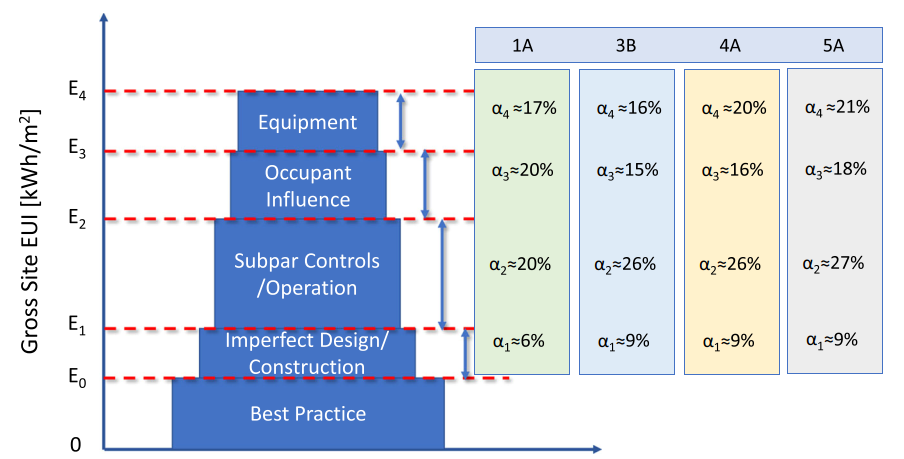
\includegraphics[width=\linewidth]{figures/Integrated technical building energy-saving potential of a typical medium office building in the United States.png}
  \caption{Integrated building energy-saving breakdown by category and climate zone.}
  \label{fig:category-breakdown}
\end{figure}

  

\end{document}
